%----------------------------------------------------------------------------------------
%	PACKAGES AND OTHER DOCUMENT CONFIGURATIONS
%----------------------------------------------------------------------------------------

\documentclass[9pt]{developercv}
\usepackage{graphicx}
\usepackage[export]{adjustbox}
%----------------------------------------------------------------------------------------

\begin{document}

%----------------------------------------------------------------------------------------
%	TITLE AND CONTACT INFORMATION
%----------------------------------------------------------------------------------------

\begin{minipage}[t]{0.3\textwidth}
	\vspace{-\baselineskip}
	\colorbox{black}{{\Huge\textcolor{white}{\textbf{\MakeUppercase{Ionut Daniel}}}}}
	
	\colorbox{black}{{\Huge\textcolor{white}{\textbf{\MakeUppercase{Fagadau}}}}}
	
	\vspace{6pt}
	
	{\Large 17 Gennaio 1999 \\ Dorohoi, Romania}
\end{minipage}
\begin{minipage}[t]{0.22\textwidth} 
	\vspace{-\baselineskip}
	
	\icon{MapMarker}{12}{Trecate, Novara}\\
	\icon{Phone}{12}{+39 3890989121}\\
\end{minipage}
\begin{minipage}[t]{0.3\textwidth}
\vspace{-\baselineskip}
\icon{At}{12}{danielfagadau@gmail.com}\\
	\icon{Linkedin}{12}{\href{https://www.linkedin.com/in/daniel-fagadau/}{daniel-fagadau}} \\	
\end{minipage}
\begin{minipage}[t]{0.2\textwidth}
\vspace{-\baselineskip}
\noindent
\centering
\vspace{-20mm}{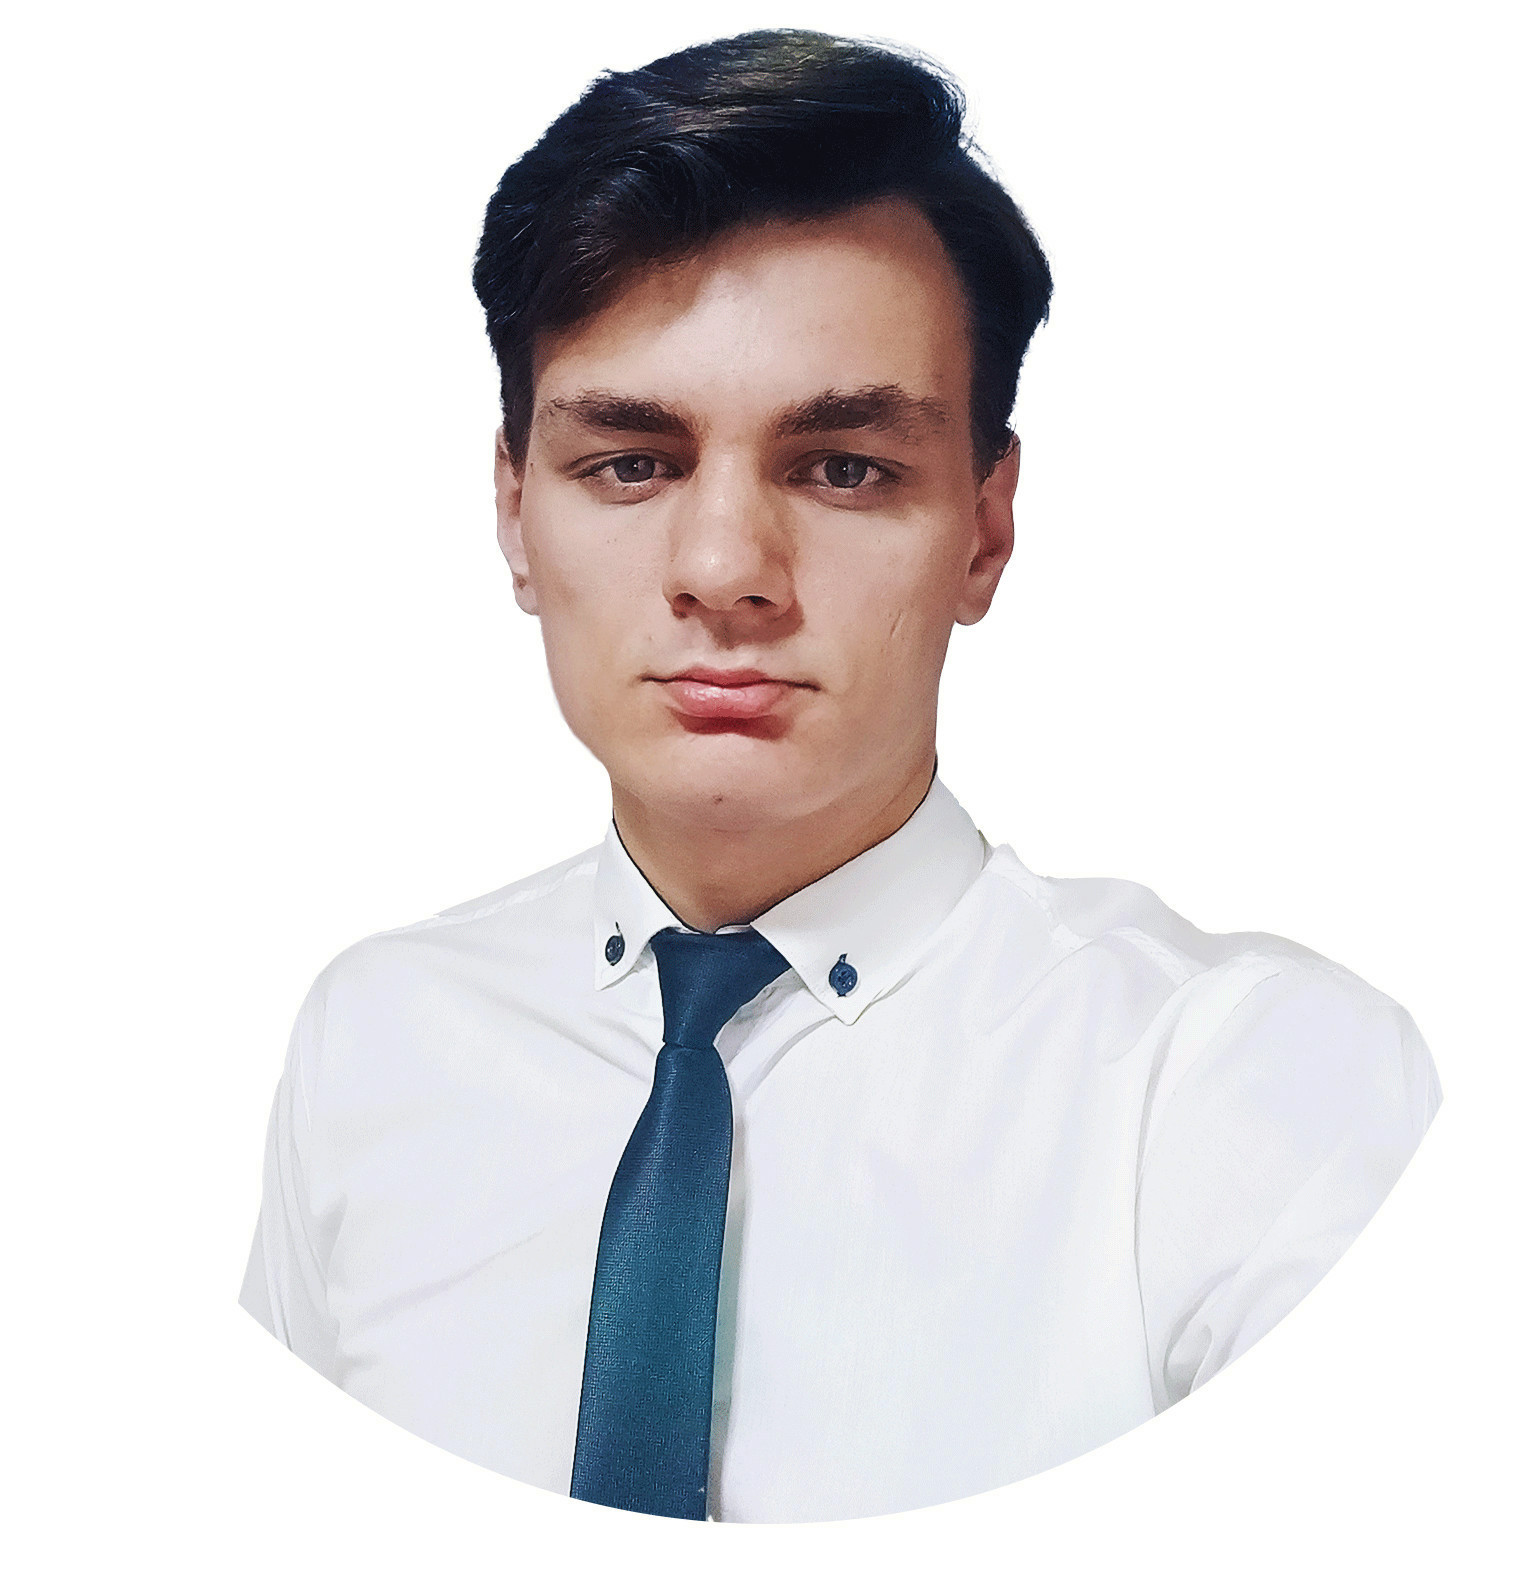
\includegraphics[scale=0.045, center]{foto_cv}}
\end{minipage}

\vspace{0.5cm}


%----------------------------------------------------------------------------------------
%	EXPERIENCE
%----------------------------------------------------------------------------------------

\cvsect{Esperienza professionale}

\begin{entrylist}
	\entry
		{Marzo 2020 \\ Presente \\\footnotesize{smart working}}
		{MindBlooming: una soluzione mobile a supporto della CBT}
		{Università degli Studi di Milano Bicocca}
		{Dopo l'iniziale periodo di stage ho deciso, assieme alla prof.ssa Daniela Micucci e al dott. Davide Ginelli, di continuare il progetto nato durante i mesi precedenti permettendomi così di approfondire ancor di più le mie conoscenze sul mondo mobile andando ad esplorare anche aspetti meno comuni in un approccio iniziale ma presenti in prodotti finiti. Inoltre, il progetto prevedeva la collaborazione col dipartimento di Psicologia UniMiB, aspetto che mi ha permesso di sviluppare molto le mie capacità di lavorare in team, di comunicare e di capire le richieste. \\ \texttt{Java}\slashsep\texttt{Dart}\slashsep\texttt{Flutter}}
	\entry
		{Dicembre 2020 \\ Marzo 2020\\\footnotesize{smart working}}
		{Stage sviluppo cross-platform con Flutter}
		{Università degli Studi di Milano Bicocca}
		{Lo stage prevedeva lo sviluppo di un applicazione multi-piattaforma a sostegno della terapia cognitivo comportamentale utilizzando il framework Flutter. Questa esperienza mi ha permesso di acquisire ottime conoscenze dell'ambiente mobile, soprattutto sul funzionamento di Android grazie anche al corso di Programmazione di Dispositivi Mobile. È stata un'esperienza utile per sviluppare alcune soft skills come il problem solving, il lavoro autonomo, il self-learning e l'adattabilità a soluzioni nuove. Avendo inoltre eseguito una sorta di sprint settimanali durante lo stage ho migliorato anche le mie capacità di lavorare per obiettivi e di pianificazione e organizzazione.  \\ \texttt{Java}\slashsep\texttt{Dart}\slashsep\texttt{Flutter}}
	\entry
		{3/9/2018  21/9/2018}
		{Elmec SmartCollege}
		{Elmec Informatica S.P.A. - Varese}
		{Dopo il diploma ho svolto un corso intensivo di formazione su gestione clienti, web design, sviluppo web e cross-platform, UI e UX Design a diretto contatto con i relativi reparti di Elmec. \\ \texttt{node.js}\slashsep\texttt{Vue.js}\slashsep\texttt{React Native}}
	\entry
		{2016 -- 2018\\\footnotesize{part time}}
		{Grafica Sito web \& Gestione database}
		{Indieversus - Novara}
		{Durante il triennio liceale ho anche lavorato per una community indipendente svolgendo sia attività di grafica pubblicitaria e di UI Design che di sviluppo e mantenimento del sito web. Durante questo periodo ho avuto modo di acquisire anche alcune competenze trasversali come la buona gestione del tempo e la capacità di adattamento a contesti lavorativi diversi. \\ \texttt{HTML}\slashsep\texttt{PHP}\slashsep\texttt{JS}\slashsep\texttt{Photoshop}\slashsep\texttt{After Effects}}
	\entry
		{2016 -- 2018}
		{Alternanza Scuola Lavoro}
		{ITIS G. Fauser - Novara}
		{Sono state svolte varie esercitazioni CISCO, esperienze di laboratorio ed incontri informativi su Industria 4.0, Internet of Things e sviluppi futuri dell'informatica. \\ \texttt{C}\slashsep\texttt{C\#}\slashsep\texttt{C++}\slashsep\texttt{Cisco Packet Tracer}}
\end{entrylist}

%----------------------------------------------------------------------------------------
%	EDUCATION
%----------------------------------------------------------------------------------------

\cvsect{Istruzione e formazione}

\begin{entrylist}
	\entry
		{2018 -- 2021}
		{Laurea Triennale}
		{Università Degli Studi di Milano Bicocca}
		{Conseguimento laurea triennale in Informatica. Media attuale: 28.263/30}
	\entry
		{2015 -- 2018}
		{Diploma esame di stato - profilo informatico}
		{ITIS G. Fauser - Novara}
		{Voto: cento/centesimi}
	\entry
		{2013 -- 2015}
		{Biennio profilo informatico}
		{ITIS H. Hertz - Roma}
		{Ho svolto i primi due anni di liceo a Roma.}
\end{entrylist}

%----------------------------------------------------------------------------------------
%	ADDITIONAL INFORMATION
%----------------------------------------------------------------------------------------

\begin{minipage}[t]{0.3\textwidth}
	\vspace{-\baselineskip}

	\cvsect{Lingue}
	
	\textbf{Inglese} - C1 certificato CAE\\
	\textbf{Italiano} - Lingua madre\\
	\textbf{Rumeno} - Lingua madre
\end{minipage}
\hfill
\begin{minipage}[t]{0.3\textwidth}
	\vspace{-\baselineskip}
	
	\cvsect{Borse di Studio}
	
	\textbf{TalentAward} - Elmec, 2018 \\
	\textbf{Giuseppe Sironi} - G. Fauser, 2017
\end{minipage}
\hfill
\begin{minipage}[t]{0.3\textwidth}
	\vspace{-\baselineskip}
	
	\cvsect{Patente di guida}
	
	B
\end{minipage}

%----------------------------------------------------------------------------------------

\vskip 0.8em
\cvsect{Dati Personali}

Autorizzo il trattamento dei miei dati personali ai sensi del Decreto Legislativo 30 giugno 2003, n. 196 "Codice in materia di protezione dei dati personali”.

\end{document}
